\documentclass[runningheads]{llncs}
\pagestyle{plain}
\usepackage[T1]{fontenc}
\usepackage{amsmath,amssymb}
\usepackage{booktabs}
\usepackage{array}
\usepackage{graphicx}
\usepackage[table]{xcolor}
\usepackage{tikz}
\usetikzlibrary{automata,positioning,arrows.meta}
\usepackage{hyperref}
\hypersetup{hidelinks}

\newcommand{\F}{\mathbb{F}}
\newcommand{\DDT}{\mathrm{DDT}}
\newcommand{\LAT}{\mathrm{LAT}}
\newcommand{\BCT}{\mathrm{BCT}}
\newcommand{\Sig}{\Sigma}
\newcommand{\re}[1]{\texttt{#1}}
\newcommand{\wt}{\mathrm{wt}}

\begin{document}

\title{An Automaton-Theoretic Representation of\\ Difference Distribution Tables}
\titlerunning{An Automaton-Theoretic Representation of DDTs}
\author{Anonymous Submission}
\authorrunning{Anonymous Submission}
\institute{}
\maketitle

\begin{abstract}
Differential cryptanalysis, introduced by Biham and Shamir, centers on the
difference distribution table (DDT) of an S-box. For an $n$-bit S-box the table
is a dense $2^{n}\times 2^{n}$ matrix, and even when it fits in memory the
cryptanalytic tasks performed over it are each implemented as an ad-hoc scan,
written anew for every analysis. Other approaches encode the DDT into a generic
solver (MILP, SAT) for a specific analysis, or compress it with generic
sparse-matrix data structures for storage; as far as we know, none offers a uniform, queryable
representation of the table itself. We argue that the right abstraction for the DDT is not a matrix but
a formal language: by recursively partitioning the table
into quadrants, every cell is identified with a unique word over a quaternary
alphabet $\Sigma = \{\texttt{0},\texttt{1},\texttt{2},\texttt{3}\}$, the nonzero entries form a
regular language $L(D)$, and a quaternary analogue of multi-terminal binary
decision diagram reduction makes the recognizing automaton canonical. The ad-hoc scans then collapse into a single uniform recipe: any property
definable over $\Sigma$ becomes a query automaton $Q$ and the matching entries are recovered by a joint traversal of $D$ and $Q$ that
never materializes the matrix. We develop this query calculus, validate seven
query families against exhaustive search, and show that the same construction
and calculus apply verbatim to the linear approximation and boomerang
connectivity tables, unifying differential, linear, and boomerang queries under
a single engine. We evaluate the construction on the entire
SageMath S-box library, $288$ S-boxes from $n=3$ to $9$ with every automaton
verified cell-by-cell against the dense table. We also build the automaton for the 16-bit FI function of MISTY1, well beyond the sizes the SageMath library covers, at a cost comparable to the matrix representation it replaces. The resulting automaton stays within a small factor of
sparse-bitmap encodings on unstructured S-boxes and improves on them by up to
an order of magnitude on highly structured ones.
\keywords{Differential cryptanalysis \and Difference distribution table \and
Decision diagrams \and Finite automata \and S-box.}
\end{abstract}

\section{Introduction}

Differential cryptanalysis, introduced by Biham and Shamir~\cite{BihamAndShamir1991}, is one
of the most influential statistical attacks against symmetric-key primitives. Its
central insight is that the propagation of a chosen input difference through an
iterated cipher is far from uniform, and that pairs of input and output
differences that occur with high probability can be combined into multi-round
trails that distinguish the cipher from a random permutation or recover key
material. In the decades since its introduction, the technique has been refined
into a broad family of variants, including truncated, higher-order, impossible,
and boomerang differential attacks. All of them share the same underlying object:
the difference distribution table of the cipher's nonlinear components, which
records the frequency with which each output difference is produced by each input
difference.

Most cryptanalytic tasks do not need every cell at once: they need
to extract the small subset of entries that satisfy some criteria.
Examples are pervasive in the literature, including enumerating all impossible
differentials of an S-box, listing every $(a,b)$ that achieves the differential
uniformity, isolating truncated differentials in which only a few input bits are
active, identifying entries that satisfy a linear relation imposed by the
surrounding cipher, and filtering transitions whose probability lies above a
chosen threshold. In the standard matrix view, each of these queries is solved by
an ad-hoc procedure, written anew for every analysis, and each shares the same
unavoidable lower bound: a full or partial sweep of the table.

In this paper, we argue that the right abstraction for the DDT is not a matrix but
a formal language. By recursively partitioning the table into quadrants, every
cell is identified with a unique word over a quaternary alphabet, and the set of
words that correspond to nonzero entries forms a regular language $L(D)$. This
language is recognized by a finite automaton whose terminal states carry the
differential multiplicities, and whose structure is canonical once a quaternary
analogue of multi-terminal binary decision diagram reduction is applied. The
resulting representation exposes the structural regularities of the table:
both the abundance of zero entries common to every S-box DDT and its
specific algebraic redundancies in a form that the query calculus in
Section~\ref{sec:applications} can act on directly.

The focus of this work is the querying capability that the language-theoretic
view unlocks. Once the DDT is encoded as a
regular language, any subset of entries definable by a regular condition over the
alphabet $\Sigma = \{\texttt{0},\texttt{1},\texttt{2},\texttt{3}\}$ becomes a regular language in its own right, and can
be intersected with $L(D)$ using standard automata-theoretic constructions. The
disparate ad-hoc scans listed above all collapse into a single uniform recipe:
write the property as a regular expression, compile it into a query automaton,
intersect with the DDT automaton, and enumerate the resulting language. Truncated
differentials, impossible differentials, fixed-bit differentials, entries of
extremal probability, and many other targets that have historically required
specialized code are recovered as one-line queries. Importantly, this also lifts
queries from a per-cell cost to a cost proportional to the size of the
intersection automaton, so the dense matrix is never enumerated.

We make three contributions. First, we describe the construction and canonical
reduction of the DDT automaton (Section~\ref{sec:auto}) and evaluate it on the
\emph{entire} SageMath S-box library~\cite{Sage2026}, $288$ S-boxes spanning $n=3$ to
$9$, every reported automaton verified cell-by-cell against its dense table, and
on the $16$-bit FI function of MISTY1, beyond the sizes the library covers
(Section~\ref{sec:results}). Second, we develop the query calculus and
validate seven query families against exhaustive search
(Section~\ref{sec:applications}). Third, we observe that nothing in the
construction is specific to the DDT, and show that the linear approximation table
(LAT) and boomerang connectivity table (BCT) are represented and queried by the
same machinery, placing differential, linear, and boomerang analysis on a common
footing (Section~\ref{sec:beyond}). Section~\ref{sec:conclusion} provides concluding remarks and suggests directions for future work. A
self-checking artifact reproduces every measurement.\footnote{https://anonymous.4open.science/r/submission-123456/}

\section{Preliminaries}
\label{sec:prelim}

This section establishes the concepts and notation used throughout, covering the
relevant properties of the cryptanalytic tables, finite automata, and decision
diagrams.

\subsection{Differential cryptanalysis and its tables}

Let $F:\F_2^{n}\to\F_2^{m}$ be a vectorial Boolean function (an S-box). For an
input difference $a$, the derivative of $F$ in direction $a$ is
$D_aF(x)=F(x+a)+F(x)$; counting how often each output difference occurs gives the
difference distribution table.

\begin{definition}[Difference distribution table]
The difference distribution table of $F$ is a $2^n \times 2^m$ matrix where the entry at row $a \in \mathbb{F}_{2^n}$ and column $b \in \mathbb{F}_{2^m}$ is defined as:

    \begin{equation}
        DDT_{F}[a, b] = \big|\{x \in \mathbb{F}_{2}^{n} \mid D_{a}F(x) = b\}\big|.
    \end{equation}
\end{definition}

We assume $m=n$ throughout this work, as is the case for the permutation S-boxes that
dominate practice, and return to the rectangular case in
Section~\ref{sec:conclusion}. The most studied statistics of the DDT is the
differential uniformity, which upper-bounds an attacker's per-round success
probability and is therefore kept small by design.

\begin{definition}[Differential uniformity]
The differential uniformity of $F$, denoted by $\Delta(F)$, is the maximum number of values $x \in \mathbb{F}_{2}^{n}$ such that the derivative of $F$ with respect to $a$ equals $b$, taken over all $a \ne 0 \in \mathbb{F}_{2}^{n}$ and all $b \in \mathbb{F}_{2}^{m}$

    \begin{equation}
        \Delta(F) = \max_{a \ne 0 \in \mathbb{F}_{2}^{n}, b \in \mathbb{F}_{2}^{m}} \big| \{x \in \mathbb{F}_{2}^{n} : D_{a}F(x) = b\} \big|.
    \end{equation}
\end{definition}

Designs optimized exclusively for low uniformity often acquire strong algebraic
structure, and such structure has itself been exploited in algebraic and
higher-order attacks~\cite{JakobsenAndKnudsen1997,CourtoisAndPieprzyk2002,CanteautAndVideu2002}; for that reason, several cryptanalytic tasks need
information beyond the single maximum, captured by the differential spectrum.

\begin{definition}[Differential spectrum]
The differential spectrum of $F$ is the multiset of values

    \begin{equation*}
        \big| \{ x \in \mathbb{F}_{2}^{n} \mid D_{a}F(x) = b \} \big|
    \end{equation*}
    over all $a \neq 0 \in \mathbb{F}_{2}^{n}$ and $b \in \mathbb{F}_{2}^{m}$. The elements in this multiset are represented by $\omega_{i}$, where each $\omega_{i}$ denotes the number of non-trivial differentials $(a, b)$ that occur $i$ times in $F$.
\end{definition}

Zero entries of the DDT are the \emph{impossible differentials}: a transition that
cannot occur immediately discards a key guess reached during partial decryption,
which is the backbone of impossible-differential cryptanalysis. Throughout, the
trivial differential $(0,0)$, whose value is always $2^{n}$, is overridden to $0$;
it carries no cryptanalytic information, and removing it increases the sparsity of
the table. A further metric that depends on which differentials are possible rather than on their frequency is the branch number. It asks for the minimum number of bits an input and an output difference pair can have active at the same time. This is the quantity a wide-trail design keeps large to force many active S-boxes per round.

\begin{definition}[Differential branch number]
The differential branch number of $F$, denoted by $\mathcal{B}(F)$, is the minimum combined Hamming weight of a pair of input and output differences,

    \begin{equation*}
        \mathcal{B}(F) = \min_{\substack{a \ne 0 \in \mathbb{F}_{2}^{n}, \; b \in \mathbb{F}_{2}^{m} \\ DDT_{F}[a, b] \ne 0}} \wt(a) + \wt(b).
    \end{equation*}
\end{definition}

Two further tables, defined here for use in Section~\ref{sec:beyond}, record the
behavior of $F$ under the other two main attack families. The linear
approximation table~\cite{Matsui1994} $\LAT_F[a,b]=|\{x:a\cdot x=b\cdot
F(x)\}|-2^{n-1}$ collects the correlations of linear approximations, with $\cdot$
the inner product over $\F_2$; its largest off-origin magnitude is the linearity.
For a permutation $F$, the boomerang connectivity table~\cite{CidEtAl2018}
$\BCT_F[a,b]=|\{x:F^{-1}(F(x)+b)+F^{-1}(F(x+a)+b)=a\}|$ makes the boomerang
switch~\cite{Wagner1999} exact, and its boomerang uniformity is
$\beta(F)=\max_{a,b\neq 0}\BCT_F[a,b]$. All three are square integer matrices
indexed by $(a,b)$; they differ only in how a cell is computed. This uniformity
of shape is what will let our construction apply to each of them without change.

\subsection{Finite automata and decision diagrams}

Two classical structures underlie what follows: deterministic finite automata,
which provide a query language, and decision diagrams, which provide a canonical
compact form. We recall both here in the minimal form we need.

A deterministic finite automaton (DFA) over an alphabet $\Sig$ is a $5$-tuple
$(Q,\Sig,\delta,q_0,A)$ with transition function $\delta:Q\times\Sig\to Q$,
initial state $q_0$, and accepting set $A$, recognizing the regular language
$L=\{w:\delta^{*}(q_0,w)\in A\}$. Regular languages are closed under union,
intersection, and complement; intersection is realized by the product
construction, whose reachable part is what a joint traversal explores.

A binary decision diagram (BDD)~\cite{Akers1978,Lee1959} is a rooted directed acyclic
graph whose internal nodes are labeled by a variable and have two children;
evaluation follows the \texttt{low} or \texttt{high} child according to the bit
read. Bryant~\cite{Bryant1986} showed that fixing a total variable order and applying
two reduction rules, merge isomorphic subgraphs and delete a node whose children
coincide, yield the reduced ordered BDD, which is canonical and minimal. A
multi-terminal BDD (MTBDD)~\cite{FujitaEtAl1997} relaxes the terminals from $\{0,1\}$ to an
arbitrary finite set, so that an integer-valued matrix indexed by Boolean
variables is represented by a single canonical diagram. The correspondence between
such diagrams and automata is classical~\cite{KimuraAndClarke1990}; it is what lets us treat
the diagram as a language recognizer.

\section{An Automaton-Theoretic Representation of DDTs}
\label{sec:auto}

We propose a DDT representation based on automata theory, resting on the
hypothesis that the derivatives of the functions used as S-boxes in real ciphers
are not random, but possess significant structural regularities that the
automaton view can both compress and query. We first identify the redundancy
that a dense matrix fails to exploit, then describe the construction of the
automaton and its reduction.

\subsection{Structural redundancy in DDTs}
\label{sec:redundancy}

For an $n$-bit S-box, representing the DDT as a matrix requires $2^{2n}$ elements,
which quickly becomes prohibitive both for storage and for in-memory analysis as
$n$ grows. The inefficiency of this representation is the result of two kinds of
redundancy. The first is the \emph{general} redundancy present in every DDT:
because the number of distinct differential values is far smaller than the number
of cells, many cells share a value, and at least half of all entries are zero. The
second is the \emph{specific} redundancy induced by the structure of the S-box,
which manifests as the frequent repetition of small identical blocks throughout
the table.

This specific redundancy is already visible in the DDT of the PRESENT
S-box~\cite{BogdanovEtAl2007}, shown
in Table~\ref{tab:present}. Here the table is partitioned into $2\times 2$ blocks
and each block is shaded by how often its pattern occurs, with more frequent
patterns darker. Although the $64$ blocks could in principle realize a great many
distinct patterns, $25$ of them fall into just three patterns, the all-zero
block alone occurs $11$ times, and only $16$ distinct block patterns appear in
total. This repetition is precisely what a quadrant-based encoding can share, and
it is the source of the compression measured in Section~\ref{sec:results}.

\begin{table}[t]
\centering
\caption{The DDT of the PRESENT S-box, partitioned into $2\times2$ blocks and
shaded by pattern frequency (darker $=$ more frequent; zero entries shown as a
dot). Twenty-five of the $64$ blocks fall into the three most common patterns.}
\label{tab:present}
\setlength{\tabcolsep}{0pt}\renewcommand{\arraystretch}{1.1}
\footnotesize
\input{present_table.tex}
\end{table}

\subsection{Constructing a finite automaton from a DDT}

We present the construction as a transformation of the DDT since it makes the encoding easy to state and picture. In practice the automaton is built directly from the S-box definition and the DDT is never materialized.

To transform a DDT into a finite automaton we employ an encoding used for
quadtrees and image patterns~\cite{BerstelAndNaitAbdallah,BerstelAndMorcrette}. Let $\Sig=\{0,1,2,3\}$ be a
quaternary alphabet. The whole matrix is assigned the empty word $\varepsilon$; we
then partition the $2^{n}\times 2^{n}$ matrix into four equal quadrants and assign
a distinct symbol of $\Sig$ to each. Applied recursively, a sub-matrix labeled
$w$ has its four quadrants labeled $w0,w1,w2,w3$ for the top-left, top-right,
bottom-left, and bottom-right quadrant, until single cells are reached and receive
words of length $n$. The subset of words mapping to nonzero entries is the
\emph{language of the DDT}, written $L(D)$. Figure~\ref{fig:enc} illustrates the
scheme for an $8\times 8$ table.

The symbol read at each level encodes one bit of the row index $a$ and one of the
column index $b$. Writing the symbol as the pair $(a_i,b_i)$, we set
\begin{equation}\label{eq:enc}
  \sigma = 2a_i + b_i,
\end{equation}
so that the input bit is the high bit and the output bit the low bit of $\sigma$,
and the bits are read in the interleaved order $a_{n-1},b_{n-1},\dots,a_0,b_0$,
most significant pair first. For instance, $a=101_2$ and $b=011_2$ give the bit
pairs $(1,0),(0,1),(1,1)$ and hence the word $\re{213}$. This single convention is
used everywhere below; in particular, an input-active position ($a_i=1$) uses the
symbols $\{2,3\}$ and an output-active position ($b_i=1$) uses $\{1,3\}$.

\begin{figure}[t]
\centering
\resizebox{0.92\textwidth}{!}{%
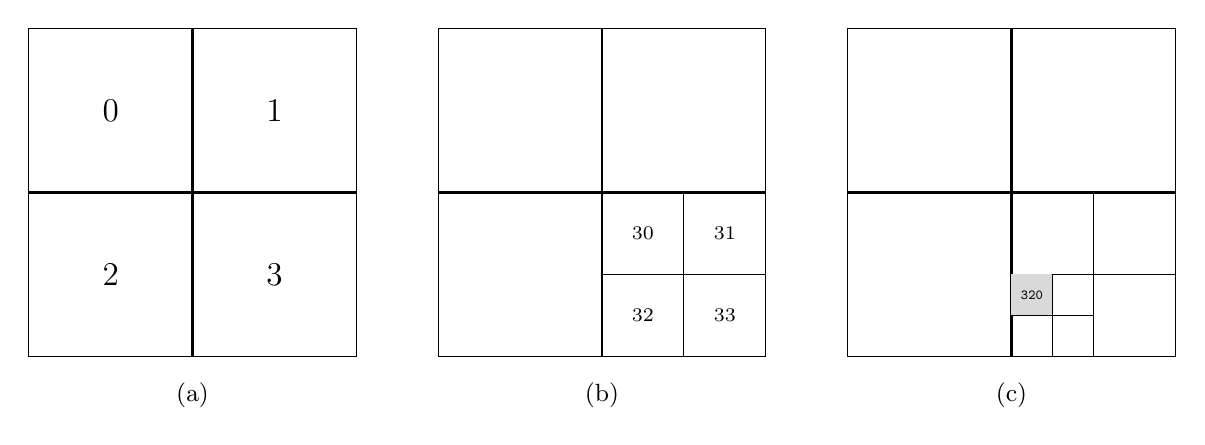
\begin{tikzpicture}[scale=0.52,every node/.style={font=\small}]
 \draw (0,0) rectangle (8,8);
 \draw[thick] (4,0)--(4,8); \draw[thick] (0,4)--(8,4);
 \node at (2,6) {\large 0}; \node at (6,6) {\large 1};
 \node at (2,2) {\large 2}; \node at (6,2) {\large 3};
 \node[below] at (4,-0.4) {(a)};
 \begin{scope}[xshift=10cm]
   \draw (0,0) rectangle (8,8);
   \draw[thick] (4,0)--(4,8); \draw[thick] (0,4)--(8,4);
   \draw (6,0)--(6,4); \draw (4,2)--(8,2);
   \node at (5,3) {\scriptsize 30}; \node at (7,3) {\scriptsize 31};
   \node at (5,1) {\scriptsize 32}; \node at (7,1) {\scriptsize 33};
   \node[below] at (4,-0.4) {(b)};
 \end{scope}
 \begin{scope}[xshift=20cm]
   \draw (0,0) rectangle (8,8);
   \draw[thick] (4,0)--(4,8); \draw[thick] (0,4)--(8,4);
   \draw (6,0)--(6,4); \draw (4,2)--(8,2); \draw (4,1)--(6,1); \draw (5,0)--(5,2);
   \fill[gray!30] (4,1) rectangle (5,2);
   \node at (4.5,1.5) {\tiny\re{320}};
   \node[below] at (4,-0.4) {(c)};
 \end{scope}
\end{tikzpicture}%
}
\caption{Recursive quadrant encoding of an $8\times 8$ DDT. (a) the table split
into four quadrants, each a symbol of $\Sig$; (b) each quadrant split again, so
sub-quadrants receive length-two words; (c) the highlighted cell encoded as
\re{320}.}
\label{fig:enc}
\end{figure}

Following this structural mapping, $L(D)$ is recognized by a quaternary automaton
in which each path from the initial state to a terminal corresponds to a word
$w\in\Sig^{n}$: internal states are the sub-matrices produced by the recursive
partition, and transitions are dictated by the symbols of $\Sig$. Unlike a
standard DFA, which outputs only accept or reject, this automaton must return the
DDT values, so we equip it with a function $f_D:\Sig^{n}\to\mathbb{N}$. Evaluating
a word therefore both decides whether the differential is possible and returns its
multiplicity.

\paragraph{Reduction.}
To store the automaton compactly, minimization is necessary, but classical DFA
minimization cannot be applied directly: it would merge accepting states carrying
different values. Instead we draw on the relationship between automata and
decision diagrams~\cite{KimuraAndClarke1990} and on the integer terminals of the
MTBDD~\cite{FujitaEtAl1997}, and reduce a quaternary variant of a decision diagram in which
each internal node $v$ has four children $E_0(v),\dots,E_3(v)$:
\begin{enumerate}
  \item terminals are shared, one per distinct value, leaving a single dead
        terminal for $0$;
  \item if $E_0(v)=E_1(v)=E_2(v)=E_3(v)$ are all terminal, node $v$ is redundant and is replaced by
        that common child;
  \item if two internal nodes \emph{at the same level} have identical children,
        they are merged.
\end{enumerate}
The level qualifier in rule~3 reflects that a node's identity in an ordered diagram
is the pair (variable, children): two nodes with the same children at different
depths are distinct, and merging them would corrupt evaluation. While the
resulting automaton is not minimal in the ordinary sense, it is minimal and
canonical for the bit order fixed by Equation~\eqref{eq:enc}, which follows from
Bryant's argument~\cite{Bryant1986} and the correspondence between diagrams and
automata~\cite{KimuraAndClarke1990}. A different order induces a different
partition and may admit a smaller automaton.

\paragraph{A worked example.}
To illustrate the construction and its reduction, consider the $3$-bit S-box of
the SEA cipher~\cite{StandaertEtAl2006}, whose DDT is shown in Table~\ref{tab:sea}. Because the S-box is
APN, its only nonzero value is $2$, and the trivial differential at $(0,0)$ is
overridden to $0$. The unreduced automaton spells out all $28$ paths to nonzero
cells. Reduction collapses the repeated structure: at the first level the
branches on symbols $0$, $1$, and $2$ lead to identically structured
sub-matrices and are grouped, immediately sparing half the storage, and at the
terminal level a single accepting state suffices for the value $2$. The reduced
automaton has nine states, the dead-state sink at index $0$, the value-$2$ sink
at index $1$, and seven internal states; in Figure~\ref{fig:sea} the dead sink
is omitted for clarity.

\begin{table}
\centering
\caption{DDT of the $3$-bit S-box of the SEA cipher (rows $a$, columns $b$). The
S-box is APN, so every nonzero entry equals $2$.}
\label{tab:sea}
\footnotesize
\begin{tabular}{c|cccccccc}
$a\backslash b$ & 000 & 001 & 010 & 011 & 100 & 101 & 110 & 111\\
\hline
000 & 0 & 0 & 0 & 0 & 0 & 0 & 0 & 0\\
001 & 0 & 2 & 0 & 2 & 0 & 2 & 0 & 2\\
010 & 0 & 2 & 2 & 0 & 0 & 2 & 2 & 0\\
011 & 0 & 0 & 2 & 2 & 0 & 0 & 2 & 2\\
100 & 0 & 0 & 0 & 0 & 2 & 2 & 2 & 2\\
101 & 0 & 2 & 0 & 2 & 2 & 0 & 2 & 0\\
110 & 0 & 2 & 2 & 0 & 2 & 0 & 0 & 2\\
111 & 0 & 0 & 2 & 2 & 2 & 2 & 0 & 0\\
\end{tabular}
\end{table}

\begin{figure}[h]
\centering
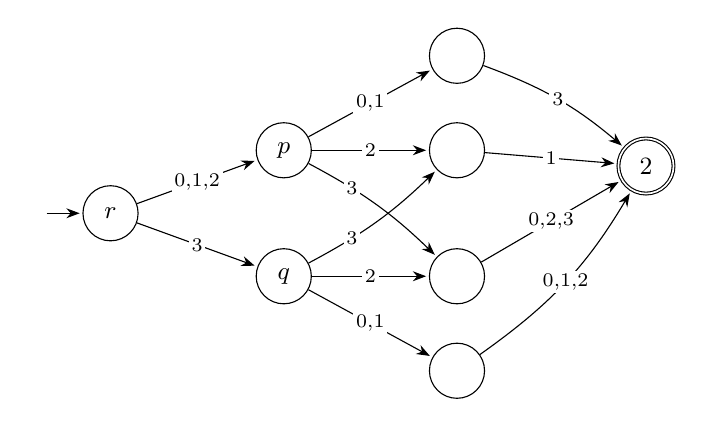
\begin{tikzpicture}[->,>=Stealth,shorten >=1pt,node distance=15mm and 20mm,
   every state/.style={draw,minimum size=7mm,inner sep=1pt,font=\small},on grid]
 \node[state,initial,initial text=] (A) {$r$};
 \node[state] (B) [above right=8mm and 22mm of A] {$p$};
 \node[state] (C) [below right=8mm and 22mm of A] {$q$};
 \node[state] (D) [above right=12mm and 22mm of B] {};
 \node[state] (E) [right=22mm of B] {};
 \node[state] (F) [right=22mm of C] {};
 \node[state] (G) [below right=12mm and 22mm of C] {};
 \node[state,accepting,double] (T) [below right=2mm and 24mm of E] {$2$};
 \tikzset{every node/.style={font=\scriptsize,fill=white,inner sep=1pt}}
 \draw (A) edge node {0,1,2} (B);
 \draw (A) edge node[swap] {3} (C);
 \draw (B) edge node {0,1} (D);
 \draw (B) edge node {2} (E);
 \draw (B) edge[bend left=8] node[pos=0.3] {3} (F);
 \draw (C) edge[bend right=8] node[pos=0.3] {3} (E);
 \draw (C) edge node[swap] {2} (F);
 \draw (C) edge node[swap] {0,1} (G);
 \draw (D) edge[bend left=10] node {3} (T);
 \draw (E) edge node {1} (T);
 \draw (F) edge node[swap] {0,2,3} (T);
 \draw (G) edge[bend right=12] node[swap] {0,1,2} (T);
\end{tikzpicture}
\caption{Reduced automaton for the SEA DDT. Edges are labeled by the symbols
taking each state to its successor; transitions to the dead state are omitted. The
double circle is the single accepting state, of value $2$. State $r$ represents the DDT matrix as whole, while $p$ and $q$ represent its immediate sub-matrices.}
\label{fig:sea}
\end{figure}

We evaluated the representation on the SageMath cryptography
library~\cite{Sage2026} (\texttt{sage.crypto.\allowbreak sboxes}), which gathers
$288$ S-boxes from the literature, all square, with widths from $n=3$ to $9$; of
these, $283$ are permutations. For each S-box we built the reduced automaton of
its DDT and verified it cell-by-cell against the dense table computed by Sage. We store the automaton as a contiguous array of $|S|$ states. Let $d$ be the number of distinct values in the table. The first $d$ entries are sink states, ordered by value while the remaining $|S|-d$ are internal states, each occupying four fields that hold the indices of its successors. A traversal that reaches a sink state stays there, since all of its four fields hold its own index, and a state is a sink exactly when its index is less than $d$. Alongside the states array we keep an auxiliary array of $d$ entries mapping each sink index to its value, in the smallest two's-complement field of size $w$ that holds them all. The same layout serves the three tables without change: nothing is assumed about how an index relates to the value it represents, so signed and odd values cost no more than even values.

\section{Applications}
\label{sec:applications}

\subsection{Computing differential properties}

The representation supports the direct computation of standard differential
metrics from the automaton alone. The differential uniformity is the largest value stored at a terminal, and the terminal set $T$, of size $|T| \le \Delta(F) + 1$, is kept ordered by value, so it is the last entry of the auxiliary array, read in $O(1)$. The differential spectrum is obtained by a depth-first traversal from the root that multiplies the number of valid transition symbols along each edge and, on reaching a terminal of value $i$, adds the accumulated path weight to the counter $\omega_{i}$, in $O(|S|\, |T|)$ time. The differential branch number is the same traversal under a different weight. Weigh each symbol by its Hamming weight and let $f(s)$ be the minimum weight of a path from $s$ to a terminal of nonzero value, with $f=\infty$ at the dead state and $f=0$ at the other terminals. Then $\mathcal{B}(F) = f(q_{0})$, from one memoized pass in $O(|S|)$. The condition $a \ne 0$ needs no encoding, since row zero is cleared before construction, so every word with $a=0$ ends at the dead state.

The spectrum and the branch number are single passes over the automaton, and the uniformity is a single lookup, so the three together cost a fixed number of traversals of $|S|$ states, while each one computed from the table costs a scan of its $2^{2n}$ cells. On AES that is $5393$ states against $65536$ cells, and on the $16$-bit FI function $119{,}506{,}234$ against $4{,}294{,}967{,}296$ (see Section~\ref{sec:results}). The construction pays the $2^{2n}$ cost once, and every property after that, in addition to the kinds of queries described in the next section, is read off the same object.

Impossible differentials are exactly the words rejected by the automaton: a differential $(a, b)$ is impossible if and only if its encoding is not in $L(D)$. For a single $(a, b)$ this $O(n)$ evaluation is not advantageous over an $O(1)$ table lookup, but as we now show, the language view pays off precisely when many entries are retrieved at once under a structural constraint.

\subsection{Complex queries via automata operations}
\label{sec:queries}

Once we built the finite automaton $D$ for the DDT, a cryptanalytic query becomes a regular
condition over $\Sig$, resolved by operations on languages. This turns the
ad-hoc search for differential properties into a uniform, language-theoretic
procedure:
\begin{enumerate}
  \item formulate the query as a regular expression $R$ over $\Sig$;
  \item compile $R$ into a finite automaton $Q$;
  \item compute the intersection of $D$ and $Q$ by a joint traversal (a lazy
        depth-first search over the two automata);
  \item enumerate the resulting language, yielding the matching DDT entries.
\end{enumerate}
Because regular languages are closed under union, intersection, and complement,
queries compose: the complement $\overline{L(D)}\cap\Sig^{n}$ is the impossible differential
language, the values stored at the terminals filter by probability, and
products of query automata express conjunctions, all without leaving the
framework. We write $a=a_{n-1}\cdots a_0$ and $b=b_{n-1}\cdots b_0$, use the
encoding~\eqref{eq:enc}, and let \texttt{.} abbreviate $\texttt{(0|1|2|3)}$.

\begin{description}
\item[Fixed input differences.] To list all possible output differences for a
  fixed input $a=0101$, for example, constrain each position to the corresponding input bit and
  leave the output free, giving $R=\re{(0|1)(2|3)(0|1)(2|3)}$ (positions with
  $a_i=0$ use $\{0,1\}$, those with $a_i=1$ use $\{2,3\}$). This replaces the
  $O(2^{n})$ row scan and is reused for other $a$ by relabeling.
\item[Truncated differentials.] To require only that the two most significant
  input bits be active, $R=\re{(2|3)(2|3)..}$. Any mask in $\{0,1,*\}$ on the
  input and output bits compiles to an automaton of $O(n)$ states; the
  active/inactive special case recovers the activity patterns underlying the
  MILP- and SAT-based active-S-box counts of Mouha et al.~\cite{MouhaEtAl2012} and the
  bounds of ciphers such as SKINNY~\cite{BeierleEtAl2016}.
\item[Impossible differentials.] These are the words rejected by $D$. Intersecting
  a pattern automaton with $\overline{L(D)}\cap\Sig^{n}$ enumerates the impossible
  cells of that pattern; e.g.\ for a $4$-bit S-box with only the least significant
  input bit active, $R=\re{(0|1)(0|1)(0|1)(2|3)}$. This is the elementary step of
  impossible-differential cryptanalysis as first applied to
      Skipjack~\cite{BihamEtAl1999} and DEAL~\cite{Knudsen1998}.
\item[Extremal-probability differentials.] Each accepting state stores its value,
  so a threshold $\tau$ selects $L(D_{\ge\tau})$, the differentials of probability
  at least $\tau\cdot 2^{-n}$, and $\tau=\Delta(F)$ yields
  those attaining the uniformity, the seed of branch-and-bound trail
  search~\cite{Matsui1995}. This constrains the value rather than the word and is
  resolved by the mechanism described below.
\item[Hamming-weight bounded differentials.] The words with $\wt(a)+\wt(b)\le w$
  are accepted by a counter automaton of $O(nw)$ states that adds each symbol's
  Hamming weight ($0$ for \re{0}, $1$ for \re{1} and \re{2}, $2$ for \re{3}).
  Single-bit-in, single-bit-out is
  $R=\re{0}^{*}\re{2}\,\re{0}^{*}\re{1}\,\re{0}^{*}\;|\;\re{0}^{*}\re{1}\,\re{0}^{*}\re{2}\,\re{0}^{*}\;|\;\re{0}^{*}\re{3}\,\re{0}^{*}$,
  supporting the wide-trail
  verification of Daemen and Rijmen~\cite{DaemenAndRijmen2020}.
\item[Linearly constrained differentials.] The diagonal case $a=b$ is
  $R=\re{(0|3)}^{n}$, since $\sigma\in\{0,3\}$ exactly when $a_i=b_i$; any
  $\F_2$-linear relation is accepted by a parity-tracking automaton with at most
  $2^{r}$ states for $r$ constraints, extracting the entries compatible with the
  linear context imposed by the surrounding cipher.
\item[Composite and comparative queries.] Boolean closure combines these freely:
  high-probability low-weight differentials are
  $L(D_{\ge\Delta/2})\cap L(\wt\le w)$, a single product. Queries also span two
  S-boxes: given $D_F$ and $D_G$, the language $L(D_F)\setminus L(D_G)$ collects
  the differentials possible for $F$ but impossible for $G$, a certificate of
  inequivalence useful when comparing candidate S-boxes during design.
\end{description}

\paragraph{Value bounds.}
The families of queries above constrain the word and are resolved by intersection. A query may instead constrain the value, and that is resolved by a second mechanism. Annotate every state $s$ with $\max(s)$, the largest value stored at a terminal reachable from $s$. A traversal then cuts any subtree whose root is a state $s$ with $\max(s)<\tau$. This annotation does not depend on $\tau$, so it is computed once and serves every threshold value. The two mechanisms are independent and compose, pruning both by symbol and value.

For every query the running time is dominated by the size of the intersection,
bounded by $|D|\cdot|Q|$ but usually far smaller, and the intersection is never
materialized: a joint traversal touches only the compressed automaton and the
small query automaton, so the memory savings of Section~\ref{sec:results} carry
over to query time.

\subsection{Experimental validation}
\label{sec:query-exp}

Section~\ref{sec:queries} gives these queries as constructions. We implemented all seven families and checked each against ground truth~\footnote{Anonymized artifact: \url{}}. Table~\ref{tab:query} reports, for the
PRESENT ($n=4$) and AES ($n=8$) DDT automata, the number of matching entries and
the number of product states the joint traversal visited, against the $256$ and
$65536$ cells of the dense tables. For every query we also computed the answer by
an exhaustive scan and confirmed set-equality; all seven families agreed exactly.

\begin{table}
\centering
\caption{Validated DDT queries. \emph{res.}\ is the number of matching entries and
\emph{prod.}\ the product states visited with value bound enabled; dense tables hold $256$ and $65536$
cells, with $|D|=39$ and $5393$. Every result equals the brute-force set.}
\label{tab:query}
\begin{tabular}{l r r @{\hspace{2.2em}} r r}
\toprule
 & \multicolumn{2}{c}{PRESENT ($n{=}4$)} & \multicolumn{2}{c}{AES ($n{=}8$)}\\
\cmidrule(lr){2-3}\cmidrule(lr){4-5}
query & res. & prod. & res. & prod.\\
\midrule
fixed input difference              & 7  & 16 & 127  & 146 \\
truncated (2 MSB input active)      & 26 & 19 & 8128 & 1403 \\
impossible (one input bit active)   & 12 & 11 & 129  & 135 \\
extremal ($=\Delta$)                & 24 & 28 & 255  & 779 \\
Hamming $\wt(a)+\wt(b)\le 2$        & 0  & 24 & 24   & 232 \\
linear $a=b$                        & 5  & 15 & 116  & 146 \\
composite ($\ge\Delta/2$, $\wt\le4$)& 63 & 49 & 1091 & 1492 \\
\bottomrule
\end{tabular}
\end{table}

The traversal visits far fewer product states than the table has cells. The AES truncated query inspects $1403$ states to enumerate $8128$ matching entries against $65536$ cells, and the structural queries stay in the low hundreds. Six of the seven constrain the word, so the intersection alone cuts them. The extremal query does not, as it accepts every word and asks only about the value, so without the bound it must walk all of $D$. The bound reduces the number of visited states from $5393$ to $779$ on AES, and the gain grows as the largest entries become rarer: on Skipjack, where only two cells have $\Delta=12$, the same query visits only $16$ states. It disappears for APN S-boxes such as SEA, where every nonzero entry already achieves $\Delta(F)$ and no subtree can be excluded, since the zero blocks were already removed in the automaton construction. The framework also surfaces structure for free: the empty PRESENT row for $\wt\le 2$ reminds us one of the design criteria of its S-box~\cite{BogdanovEtAl2007}, that no differential with one active input and one active output bit is possible.

\section{Beyond the DDT: the LAT and BCT}
\label{sec:beyond}

Nothing in Section~\ref{sec:auto} is specific to the difference distribution
table: the construction takes any square integer matrix over the quadrant
encoding. The linear approximation table and the boomerang connectivity table are
therefore represented by exactly the same reduced automaton; the only change is
the matrix itself. Their state ratios appear alongside the DDT in
Tables~\ref{tab:agg} and~\ref{tab:curated}. The LAT ratio is the lowest of the three at every width. Its values span a larger range, the AES LAT holding $17$ distinct values against the DDT's $3$. The BCT has a small value set and therefore its ratio stays close to the DDT's.

The query calculus generalizes in the same way, turning linear and boomerang
questions into the same primitive. High-bias linear approximations, which drive
Matsui's attack~\cite{Matsui1994}, are the magnitude filter $|\LAT_F[a,b]|\ge\tau$
on the LAT automaton, with $\tau$ the linearity selecting the best approximations.
Boomerang-uniformity cells, the differences that maximize the boomerang
switch~\cite{Wagner1999,CidEtAl2018}, are the value filter $\BCT_F[a,b]=\beta(F)$ on the BCT
automaton. We validated both on the PRESENT and AES tables against an exhaustive
scan (Table~\ref{tab:latbct}); as with the extremal DDT query, these are global
value filters and so scan their table automaton, which is nonetheless far smaller
than, and is built without, the dense matrix. The upshot is that a single
automaton type and a single query engine serve differential, linear, and boomerang
cryptanalysis, with the property of interest residing entirely in the small query
automaton.

\begin{table}
\centering
\caption{Validated LAT and BCT queries against the dense scan; ``lin.''\ is the
linearity and $\beta$ the boomerang uniformity. Product states are reported
against the $256$ (PRESENT) and $65536$ (AES) dense cells.}
\setlength{\tabcolsep}{3pt}
\label{tab:latbct}
\begin{tabular}{l l l r r}
\toprule
table & query & S-box & res. & prod.\\
\midrule
LAT & $|\LAT|\ge$ lin. & PRESENT (lin.\ $4$) & 36   & 53\\
LAT & $|\LAT|\ge$ lin. & AES (lin.\ $16$)    & 1275 & 17098\\
BCT & value $=\beta$ & PRESENT ($\beta{=}16$) & 2    & 43\\
BCT & value $=\beta$ & AES ($\beta{=}6$)      & 510  & 5459\\
\bottomrule
\end{tabular}
\end{table}


\section{Storage cost}
\label{sec:results}

This section measures the representation costs in two ways: the state ratio is the table entry count $2^{2n}$ divided by the number of automaton states and it is independent of how a state is stored. The byte count prices the layout of Section~\ref{sec:auto} where each index in the states array is bit-packed to $\lceil\log_{2}|S|\rceil$ bits, the smallest width that can index the array, giving a total of $|S| \cdot 4 \lceil \log_{2} |S| \rceil + d \cdot w$ bits. We report the ratio across the library, then for a selection of ciphers, and finally we compare the storage necessary against two baselines.

The library stops at $n=9$. To test the construction at a size where the table stops being practical, we implemented the FI function of MISTY1~\cite{rfc2994}, a standardized 16-bit S-box, and built its DDT automaton. In the tables that follow, FI appears as an extra row. We did not build its LAT and BCT, so their respective entries are empty.


\paragraph{State ratio by width.}
Table~\ref{tab:agg} aggregates the state ratio by S-box size. The ratio quantifies the structure in a table: the higher it is, the more the table repeats itself. The medians range from $5.2$ to $11.7$ for $n=3$ to $8$. Most of the S-boxes in the library sit at the two sizes most used in practice, with $215$ instances at $n=4$ and $58$ at $n=8$, with the latter, which we examine below, having the widest spread, from $11.5$ to $273.1$. The two largest instances stand apart, at $217.9$ for the single $9$-bit S-box and $35.9$ for FI, both above every median below them, so the ratio does not degrade as the table grows. Neither the LAT nor the BCT ratio exceeds the DDT ratio at any width, for the reason given in Section~\ref{sec:beyond}.

\begin{table}[h]
\centering
\caption{State ratio (cells/states) over the SageMath S-box
library and our implementation of MISTY1's FI function, by width, as median~[min--max]. The BCT is restricted to the $283$
permutations in the library.}
\setlength{\tabcolsep}{3pt}
\label{tab:agg}
\begin{tabular}{r r c c c}
\toprule
$n$ & \#S-boxes & DDT & LAT & BCT\\
\midrule
3 & 3   & 7.1~[4.9--9.1]    & 3.8~[3.6--5.8]   & 7.1~[4.9--9.1]\\
4 & 215 & 5.2~[4.6--8.8]    & 3.8~[3.0--5.8]   & 3.9~[3.2--8.3]\\
5 & 7   & 10.7~[9.6--11.0]  & 6.6~[6.2--6.7]   & 5.7~[5.1--11.0]\\
6 & 3   & 11.5~[10.7--11.5] & 8.2~[3.9--9.5]   & 11.5~[10.3--11.5]\\
7 & 1   & 10.8              & 4.4              & 8.4\\
8 & 58  & 11.7~[11.5--273.1]& 3.9~[3.4--69.8]  & 10.6~[8.6--107.3]\\
9 & 1   & 217.9             & 75.6             & 27.4\\
16 & 1   &  35.9          & ---             & ---\\
\bottomrule
\end{tabular}
\end{table}

\paragraph{Selected ciphers.}
Table~\ref{tab:curated} lists a selection of well-known S-boxes with the state count and DDT, LAT and BCT ratios for each. Two factors set the state count. The first is the differential spectrum, whose distinct values fix the number of terminals. The second is where those values fall in the table, which decides how many of the remaining states can be shared. For example, CSS and Safer both have $\Delta=128$, but CSS needs $240$ states and Safer $5{,}653$. Conversely, Noekeon and PRESENT have the same differential spectrum, but $32$ and $39$ states respectively. The full per-S-box results
for all $288$ S-boxes accompany the artifact.

\begin{table}[h]
\centering
\caption{Reduced DDT automaton for selected S-boxes: state count and state ratio,
with the LAT and BCT ratios of the same S-box (Section~\ref{sec:beyond}).}
\setlength{\tabcolsep}{3pt}
\label{tab:curated}
\small
\begin{tabular}{l r r r r r r}
\toprule
S-box & $n$ & $\Delta$ & States & DDT$\times$ & LAT$\times$ & BCT$\times$\\
\midrule
SEA            & 3 & 2   & 9    & 7.1  & 3.8  & 7.1\\
PRESENT        & 4 & 4   & 39   & 6.6 & 4.9  & 5.8\\
Noekeon        & 4 & 4   & 32   & 8.0  & 4.3  & 8.3\\
Ascon          & 5 & 8   & 107  & 9.6  & 6.2  & 5.1\\
APN (6-bit)    & 6 & 2   & 356  & 11.5 & 9.5  & 11.5\\
WAGE           & 7 & 8   & 1,516 & 10.8 & 4.4  & 8.4\\
AES            & 8 & 4   & 5,393 & 12.2 & 3.8  & 12.0\\
Camellia       & 8 & 4   & 5,387 & 12.2 & 3.8  & 12.0\\
Kuznyechik     & 8 & 8   & 5,590 & 11.7 & 3.8  & 10.6\\
Skipjack       & 8 & 12  & 5,650 & 11.6 & 3.8  & 10.3\\
SKINNY (8-bit) & 8 & 64  & 890   & 73.6 & 22.8 & 29.9\\
Safer          & 8 & 128 & 5,653 & 11.6 &  5.4 &  9.3\\
CSS            & 8 & 128 & 240  & 273.1& 69.8 & 107.3\\
DryGASCON256   & 9 & 128 & 1,203 & 217.9& 75.6 & 27.4\\
MISTY1 FI   & 16 & 20 & 119,506,234 & 35.9 & --- & ---\\
\bottomrule
\end{tabular}
\end{table}

\paragraph{Storage comparison.}
Table~\ref{tab:memory} translates these state counts into bytes and compares the
automaton against two baselines. \emph{Dense} stores every cell using
$\lceil\log_2(\Delta/2+1)\rceil$ bits, the minimum needed for the value range and
the strongest matrix representation that retains $O(1)$ random access.
\emph{Bitmap} stores a $2^{2n}$-bit presence map plus, for each nonzero cell, a
$\lceil\log_2 d\rceil$-bit index into an array of the $d$ distinct values; it
exploits the abundance of zeros but not the deeper structure of the table. A
state costs $4\lceil\log_{2}|S|\rceil$ bits, so the comparison turns on the
state ratio. The automaton stays within a small factor of the bitmap, at $377$~B against
$209$~B on Ascon, $34.2$~KiB against $12.0$~KiB on AES and $35.5$~KiB against
$14.7$~KiB on Kuznyechik. On highly structured S-boxes it is smaller than both:
CSS in under $1$~KiB against $56$~KiB and $8.6$~KiB, SKINNY-8 in $4.36$~KiB
against $48$~KiB and $13.6$~KiB, DryGASCON256 in $6.47$~KiB against $224$~KiB
and $44.6$~KiB. Neither baseline supports the query operations of
Section~\ref{sec:applications}.

\begin{table}[h]
\centering
\caption{Memory footprint of the bit-packed automaton against two matrix
baselines, on the same S-boxes as Table~\ref{tab:curated}. \emph{Dense} is the
bit-packed value-range minimum, $\lceil\log_2(\Delta/2+1)\rceil$ bits per cell;
\emph{bitmap} is a $2^{2n}$-bit presence map plus a small value array.
Neither baseline supports queries.}
\label{tab:memory}
\small
\setlength{\tabcolsep}{6pt}
\begin{tabular}{l r r r r r}
\toprule
S-box & $n$ & $\Delta$ & Autom. & Dense & Bitmap\\
\midrule
SEA            &  3 & 2   &        19~B  &              8~B  &     12~B \\
PRESENT        &  4 & 4   &       119~B  &             64~B  &     45~B \\
Noekeon        &  4 & 4   &        82~B  &             64~B  &     45~B \\
Ascon          &  5 & 8   &       377~B  &            384~B  &    209~B \\
APN (6-bit)    &  6 & 2   &    1.57~KiB  &          0.5~KiB  &  0.75~KiB \\
WAGE           &  7 & 8   &    8.15~KiB  &          6.0~KiB  &  3.55~KiB \\
AES            &  8 & 4   &    34.2~KiB  &         16.0~KiB  & 12.0~KiB \\
Camellia       &  8 & 4   &    34.2~KiB  &         16.0~KiB  & 12.0~KiB \\
Kuznyechik     &  8 & 8   &    35.5~KiB  &         24.0~KiB  & 14.7~KiB \\
Skipjack       &  8 & 12  &    35.9~KiB  &         24.0~KiB  & 17.6~KiB \\
SKINNY (8-bit) &  8 & 64  &    4.36~KiB  &         48.0~KiB  & 13.6~KiB \\
Safer          &  8 & 128 &    35.9~KiB  &         56.0~KiB  & 19.0~KiB \\
CSS            &  8 & 128 &    0.94~KiB  &         56.0~KiB  &  8.6~KiB \\
DryGASCON256   &  9 & 128 &    6.47~KiB  &         224.0~KiB & 44.6~KiB \\
MISTY1 FI      & 16 &  20 &  1538.6~MiB  &  2048.0~MiB & 1317.5~MiB \\
\bottomrule
\end{tabular}
\end{table}

\section{Conclusion}
\label{sec:conclusion}

We described an automaton-theoretic representation of difference distribution
tables. After outlining the memory and access limitations of the dense matrix, we
reframed the DDT as a formal language and represented it by a reduced quaternary
automaton that captures both the general and the S-box-specific redundancy of the
table. Evaluated on the full SageMath S-box library, the representation reduces
the number of stored states by a median of $5$ to $12$ times, and by up to
$273$ times for highly structured S-boxes, without any loss of information. We also built the automaton for the 16-bit FI function of MISTY1, well beyond the sizes the SageMath library covers, where the automaton, the dense matrix and a sparse bitmap all stay within the same order of magnitude, with the first being able to answer queries.

The central observation is that the language-theoretic
view turns the cryptanalytic searches performed over the table into operations on
automata. The properties that can be phrased as regular conditions over the
quadrant encoding of $(a,b)$, fixed-input and truncated differentials, impossible
differentials, extremal-probability entries, low-weight transitions, linearly
constrained pairs, and composite or cross-table queries, are all recovered
through a single joint traversal of the DDT automaton and a small query automaton,
and we validated each against exhaustive search. Because the construction is
agnostic to how a cell is computed, the same machinery serves the linear
approximation and boomerang connectivity tables, placing the three main attack
families on a common representation.

Several directions extend this work. The square-table assumption can be lifted to
rectangular $2^{n}\times 2^{m}$ tables by an uneven recursion that consumes input
and output bits at different rates. The query class can be enriched from regular to
context-free constraints, such as bounded-difference balances across rounds, by
replacing the query automaton with a pushdown automaton and adapting the joint
traversal. The same automaton can also serve as a generator of linear inequalities
for MILP-based trail search, and quantifying the trade-off between automaton size
and the number of generated inequalities is left to future work. Finally, the size
of the reduced automaton appears to capture an intrinsic notion of the structural
regularity of an S-box, and quantifying the deviation between an actual DDT and
its random or theoretically optimal counterparts through this size-based metric
is a natural analytical follow-up.

\bibliographystyle{splncs04}
\bibliography{bibliography}

% \begin{thebibliography}{99}
% \bibitem{akers} Akers, S.B.: Binary decision diagrams. IEEE Trans. Comput.
%   C-27(6), 509--516 (1978)
% \bibitem{skinny} Beierle, C., Jean, J., K\"olbl, S., Leander, G., Moradi, A.,
%   Peyrin, T., Sasaki, Y., Sasdrich, P., Sim, S.M.: The SKINNY family of block
%   ciphers and its low-latency variant MANTIS. In: CRYPTO 2016. LNCS, vol.\ 9815,
%   pp.\ 123--153. Springer (2016)
% \bibitem{quadtree} Berstel, J., Nait Abdallah, A.: Quadtrees generated by finite
%   automata. AFCET 61/62, 167--175 (1989)
% \bibitem{patterns} Berstel, J., Morcrette, M.: Compact representation of patterns
%   by finite automata. In: PIXIM 89, pp.\ 387--402 (1989)
% \bibitem{skipjack} Biham, E., Biryukov, A., Shamir, A.: Cryptanalysis of Skipjack
%   reduced to 31 rounds using impossible differentials. In: EUROCRYPT 1999. LNCS,
%   vol.\ 1592, pp.\ 12--23. Springer (1999)
% \bibitem{biham} Biham, E., Shamir, A.: Differential cryptanalysis of DES-like
%   cryptosystems. J. Cryptology 4, 3--72 (1991)
% \bibitem{present} Bogdanov, A., Knudsen, L.R., Leander, G., Paar, C., Poschmann,
%   A., Robshaw, M.J.B., Seurin, Y., Vikkelsoe, C.: PRESENT: an ultra-lightweight
%   block cipher. In: CHES 2007. LNCS, vol.\ 4727, pp.\ 450--466. Springer (2007)
% \bibitem{bryant} Bryant, R.E.: Graph-based algorithms for Boolean function
%   manipulation. IEEE Trans. Comput. C-35(8), 677--691 (1986)
% \bibitem{bct} Cid, C., Huang, T., Peyrin, T., Sasaki, Y., Song, L.: Boomerang
%   connectivity table: a new cryptanalysis tool. In: EUROCRYPT 2018. LNCS,
%   vol.\ 10821, pp.\ 683--714. Springer (2018)
% \bibitem{rijndael} Daemen, J., Rijmen, V.: The Design of Rijndael: AES---The
%   Advanced Encryption Standard. Springer (2002)
% \bibitem{mtbdd} Fujita, M., McGeer, P.C., Yang, J.C.-Y.: Multi-terminal binary
%   decision diagrams: an efficient data structure for matrix representation.
%   Formal Methods Syst. Des. 10(2/3), 149--169 (1997)
% \bibitem{kimura} Kimura, S., Clarke, E.M.: A parallel algorithm for constructing
%   binary decision diagrams. In: ICCD 1990, pp.\ 220--223 (1990)
% \bibitem{deal} Knudsen, L.R.: DEAL---a 128-bit block cipher. Technical Report 151,
%   University of Bergen (1998)
% \bibitem{lee} Lee, C.Y.: Representation of switching circuits by binary-decision
%   programs. Bell Syst. Tech. J. 38(4), 985--999 (1959)
% \bibitem{matsuilc} Matsui, M.: Linear cryptanalysis method for DES cipher. In:
%   EUROCRYPT 1993. LNCS, vol.\ 765, pp.\ 386--397. Springer (1994)
% \bibitem{matsui} Matsui, M.: On correlation between the order of S-boxes and the
%   strength of DES. In: EUROCRYPT 1994. LNCS, vol.\ 950, pp.\ 366--375. Springer
%   (1995)
% \bibitem{mouha} Mouha, N., Wang, Q., Gu, D., Preneel, B.: Differential and linear
%   cryptanalysis using mixed-integer linear programming. In: Inscrypt 2011. LNCS,
%   vol.\ 7537, pp.\ 57--76. Springer (2012)
% \bibitem{sage} The Sage Developers: SageMath, the Sage Mathematics Software
%   System. \url{https://www.sagemath.org} (module \texttt{sage.crypto.sboxes})
% \bibitem{sea} Standaert, F.-X., Piret, G., Gershenfeld, N., Quisquater, J.-J.:
%   SEA: a scalable encryption algorithm for small embedded applications. In:
%   CARDIS 2006. LNCS, vol.\ 3928, pp.\ 222--236. Springer (2006)
% \bibitem{wagner} Wagner, D.: The boomerang attack. In: FSE 1999. LNCS, vol.\ 1636,
%   pp.\ 156--170. Springer (1999)
% \bibitem{canteaut}
% Canteaut, A., Videau, M.: Degree of composition of highly nonlinear functions and applications to higher order differential cryptanalysis. In: Knudsen, L.R. (ed.) Advances in Cryptology --- EUROCRYPT 2002. LNCS, vol. 2332, pp. 518--533. Springer, Heidelberg (2002)

% \bibitem{courtois}
% Courtois, N.T., Pieprzyk, J.: Cryptanalysis of block ciphers with overdefined systems of equations. In: Zheng, Y. (ed.) Advances in Cryptology --- ASIACRYPT 2002. LNCS, vol. 2501, pp. 267--287. Springer, Heidelberg (2002)

% \end{thebibliography}

\end{document}
